\chapter{外骨骼力矩控制算法设计}
\section{引言}
早期的外骨骼系统大多使用运动轨迹追踪的控制方法,但位移控制在人机动作不一致时会产生大的作用力,从而产生人机交互的安全风险。因此外骨骼控制正越来越多的从单纯的轨迹控制,转向对穿戴者动作反应更加柔和的力矩控制。

在实际的应用中,力矩控制一般由底层控制器和上层控制器组成。上层控制器(如阻抗控制器)用来产生期望的外骨骼力矩,而底层控制器(如PID控制器)用来控制驱动器对外骨骼期望的力矩进行追踪。在这种控制策略中,期望力矩并不是事先选定好的控制目标,而是由人机交互过程中产生的动态信号。典型的上层控制器有直接力矩控制\cite{p32,p33}、阻抗控制\cite{p34}、灵敏度放大控制\cite{p35}和基于EMG信号的控制方法\cite{p36},这些上层的控制策略均需要根据穿戴者的个体特性来对控制调整参数,以达到最佳的助力效果。底层控制器的形式较为多样,如经典的PID反馈控制\cite{p27,p28}、基于逆动力学模型的前馈力矩补偿\cite{p7,p22,p29}、自适应控制\cite{p30}、迭代学习\cite{p31}等。

\begin{figure}[!htb]
    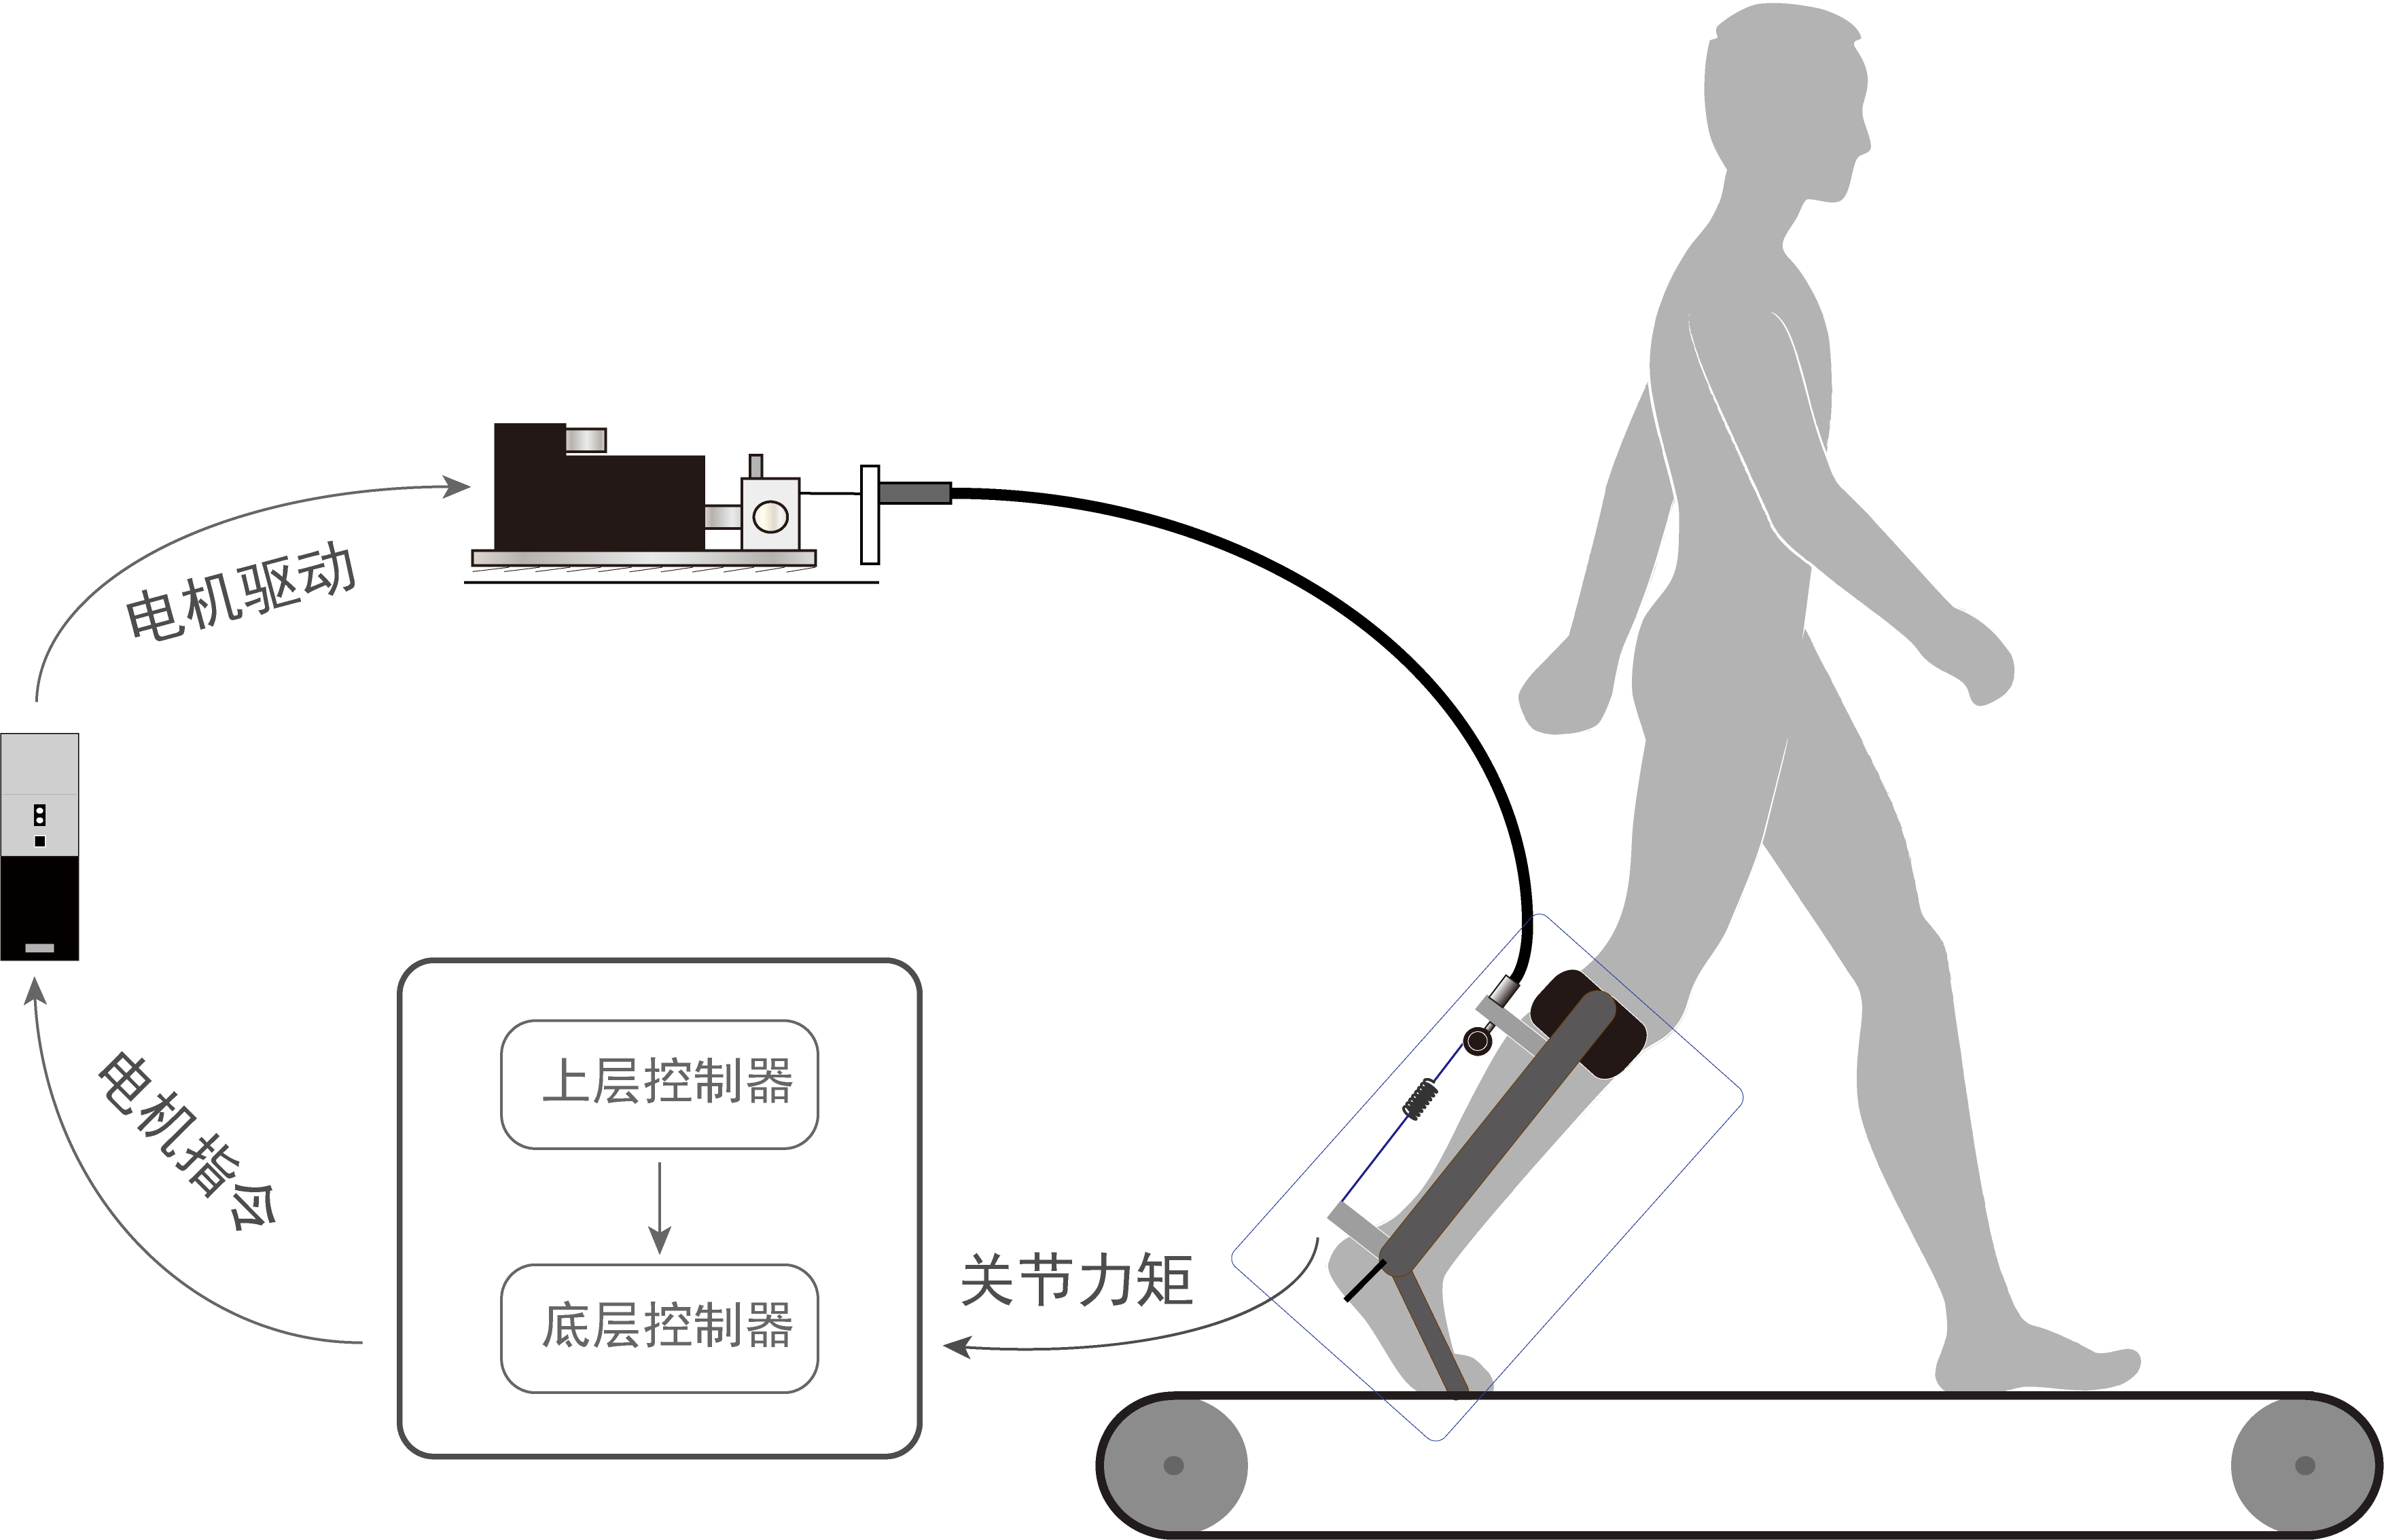
\includegraphics[width=14cm]{fig/f48.png}
    \caption{外骨骼力矩控制的硬件结构}
    \label{fig:mark}
\end{figure}

本章研究外骨骼的力矩控制算法。外骨骼力矩控制的硬件结构与组成如图3.1所示。受试者穿戴外骨骼在跑步机上以1.25m/s的速度稳定行走。通过传感系统采集外骨骼和人体的相关数据,在MicroLabBox控制器中编写上层控制器产生期望力矩曲线,设计底层控制器追踪期望力矩曲线,控制电机转动产生作用力,为穿戴者提供力矩辅助。所使用的电机为ABB公司的BSM90N-175AA,驱动器型号为MotiFlex-e180。

\section{踝关节外骨骼系统建模}

\begin{figure}[!htb]
    \label{fig:sub1}{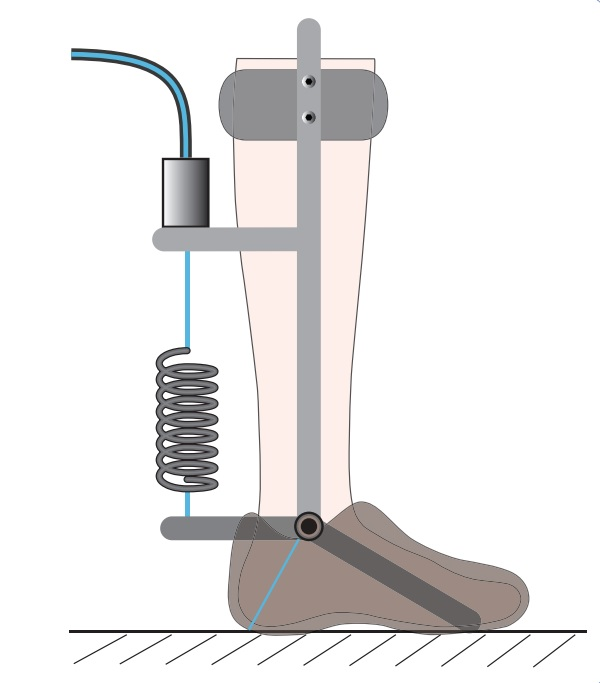
\includegraphics[width=6cm]{fig/f50.jpg}}
    \label{fig:sub2}{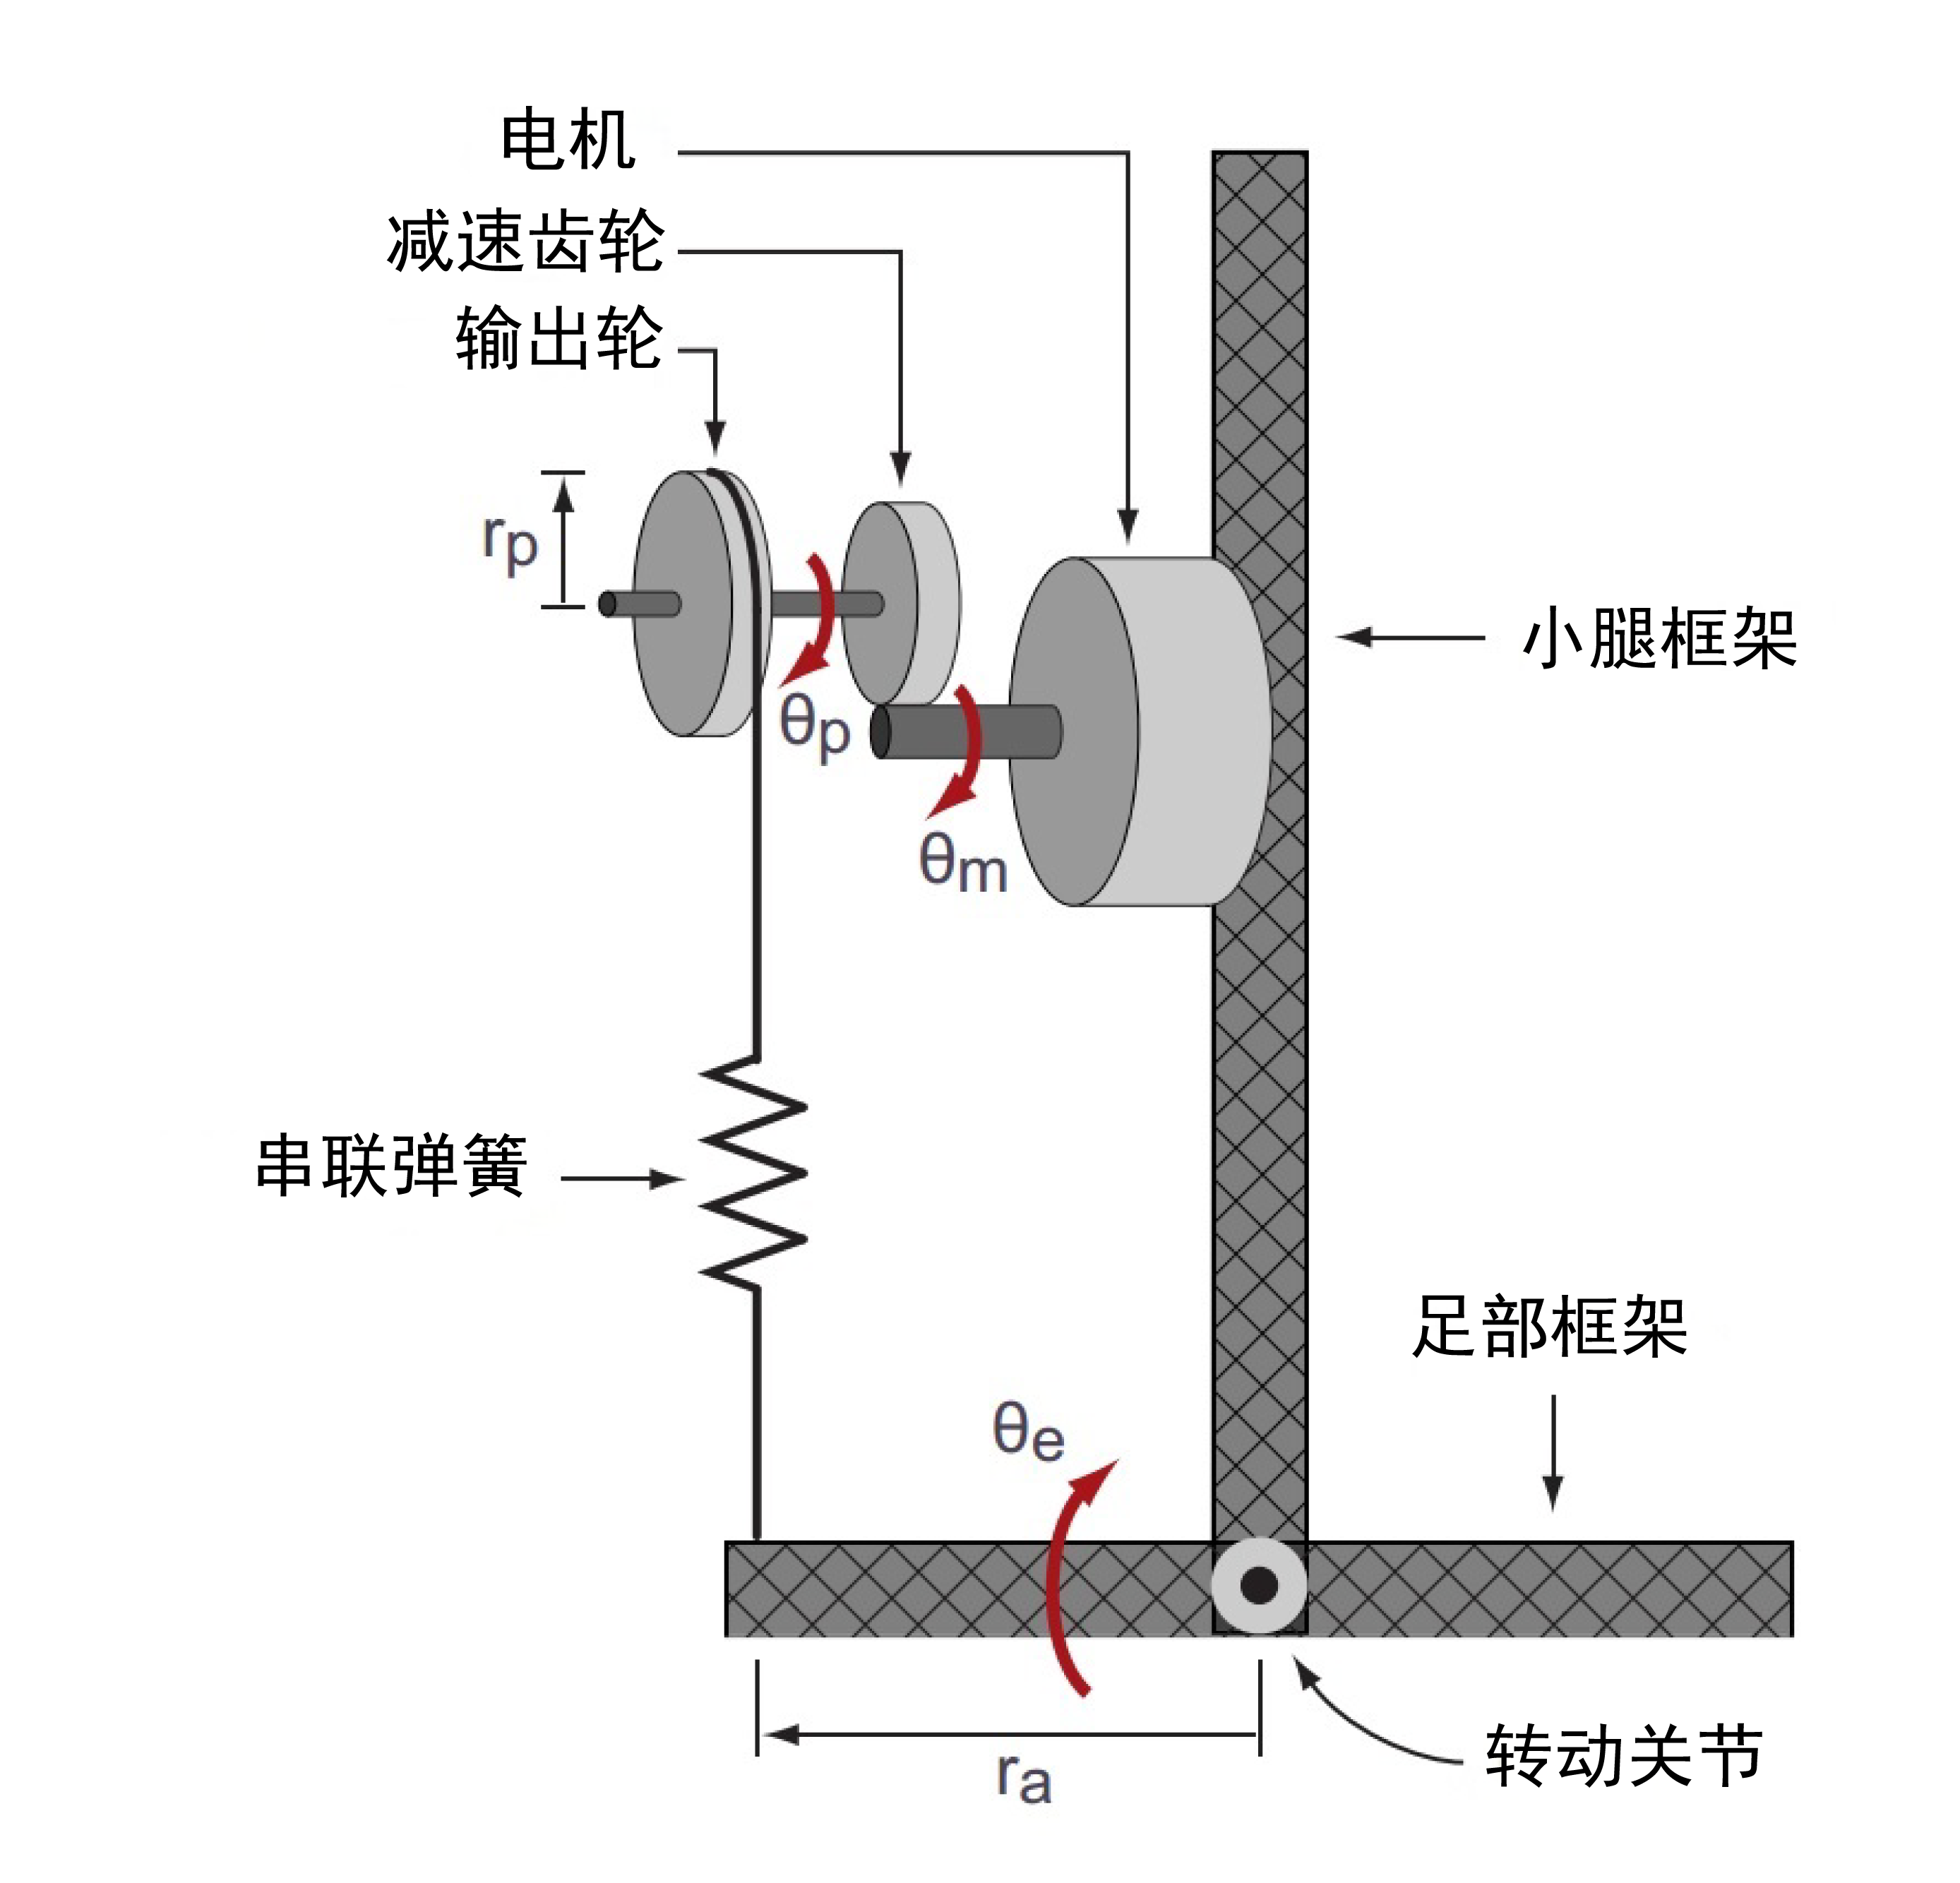
\includegraphics[width=8cm]{fig/f49.png}}
    \caption{外骨骼结构简化模型}
    \label{fig:subfigss}
\end{figure}

为了方便建模与理解,这里将电机和外骨骼视为一个整体。系统的简化模型如图3.2所示。电机通过减速箱和输出轮拉动鲍登绳,鲍登绳经串联弹簧连接外骨骼的足部框架。串联弹簧作为串联弹性驱动机构,将外骨骼与电机分离开,从而降低人机交互时的界面阻抗,提高力矩控制的柔顺度。

$\theta_m$为电机角度,$\theta_p$为减速机输出轴角度,电机齿轮减速比$N=5$,$\theta_e$为外骨骼的关节角度。

\subsection{电机动力学模型}

在忽略电枢电感影响下,建立直流电机的动力学模型:
\begin{align}
K_{a} \cdot i_{a}(t)&=I_{e} \cdot N \cdot \ddot{\theta}_{p}(t)+f_{e} \cdot N \cdot \dot{\theta}_{p}(t)+\frac{1}{N} \cdot \tau_{o}(t) \\ 
U_{a}(t)&=R_{a} \cdot i_{a}(t)+K_{b} \cdot N \cdot \dot{\theta}_{p}(t)
\end{align}

其中$K_a$为电机的转矩常数,$i_a$为电枢电流,$I_e$为电机与传动齿轮的等效转动惯量,$f_e$为电机旋转时产生的粘性摩擦系数,$\tau_o$为电机输出的力矩,$U_a$为电枢电压,$R_a$为电枢电阻,$K_b$为电机电压常数。

将式(3.1)带入(3.2)可得:
\begin{align} U_{a} &=\frac{R_{a} I_{e} N}{K_{a}} \ddot{\theta}_{p}+\left(\frac{R_{a} f_{e} N}{K_{a}}+K_{b} N\right) \dot{\theta}_{p}+\frac{R_{a}}{K_{a}} \tau_{o} \\ &=\frac{R_{a} I_{e}}{K_{a}} \ddot{\theta}_{m}+\left(\frac{R_{a} f_{e}}{K_{a}}+K_{b}\right) \dot{\theta}_{m}+\frac{R_{a}}{K_{a}} \tau_{o} 
\end{align}

当电机角加速度为零,且电枢电阻较小时,可近似认为:
\begin{align}
U_{a}=\left(\frac{R_{a} f_{e}}{K_{a}}+K_{b}\right) \dot{\theta}_{m}
\end{align}

即电机的控制电压与电机速度成线性关系

\subsection{传动模型}

鲍登线的张力$F$与电机输出的力矩$\tau_o$存在如下关系:
\begin{align}
    \tau_o = F\cdot r_p
\end{align}

其中$r_p$为电机减速器输出轮的半径。假定作用力经鲍登线传输过程中无摩擦影响,则作用在外骨骼上的力矩由如下关系:
\begin{align}
    \tau = F\cdot r_a
\end{align}

这里进一步假设踝关节角度的变化量很小,即认为外骨骼的作用力臂为常数。

\subsection{力-位置关系}

假设相对于串联弹簧而言,鲍登线的刚度系数可以忽略。由胡克定律可知:
\begin{align}
    F = K_c \cdot \Delta x_c = K_c \cdot (r_p\cdot \theta_p - r_a\cdot \theta_e)
\end{align}

式中$K_c$为等效刚度系数,$\theta_p$和$\theta_e$分别为电机输出轴角度和外骨骼踝关节角度。

\subsection{力矩-角度关系}

定义传动比系数$R$为:
\begin{align}
    R = \frac{r_a}{r_p}
\end{align}

则作用在外骨骼上的力矩可以写成如下形式:
\begin{align}
\tau &=F \cdot r_{a} \\ &=r_{p} \cdot r_{a} \cdot K_{c}\left()\theta_{p}-\frac{r_{a}}{r_{p}} \theta_{e}\right) \\ &=K_{t}\left(\theta_{p}-\theta_{e} R\right) 
\end{align}

其中传动刚度系数$K_t$定义为:
\begin{align}
    K_t = r_p\cdot r_a \cdot K_c
\end{align}

\subsection{外骨骼关节动力学模型}

对外骨骼的踝关节应用角动量定理可得:
\begin{align}
    \tau-\tau_{h}-B_{e} \cdot \dot{\theta}_{e}=I_{e} \cdot \ddot{\theta}_{e}
\end{align}

式中人体对外骨骼所有的作用力矩被简化为一个合力矩$\tau_h$,$B_e$为外骨骼关节的阻尼系数,$I_e$为外骨骼转动惯量。

\section{上层控制器设计}

本文力矩控制的上层控制器(期望力矩曲线生成器)采用基于时间的直接力矩控制。这里的时间并非绝对时间,而是步态周期百分比。具体来说是在足底开关测量得到的步态周期基础上,根据步态周期百分比进行力矩曲线的规划。基于时间的直接力矩控制,形式简单,方便实现,因此被集成在许多外骨骼系统中。

\begin{figure}[htb]
    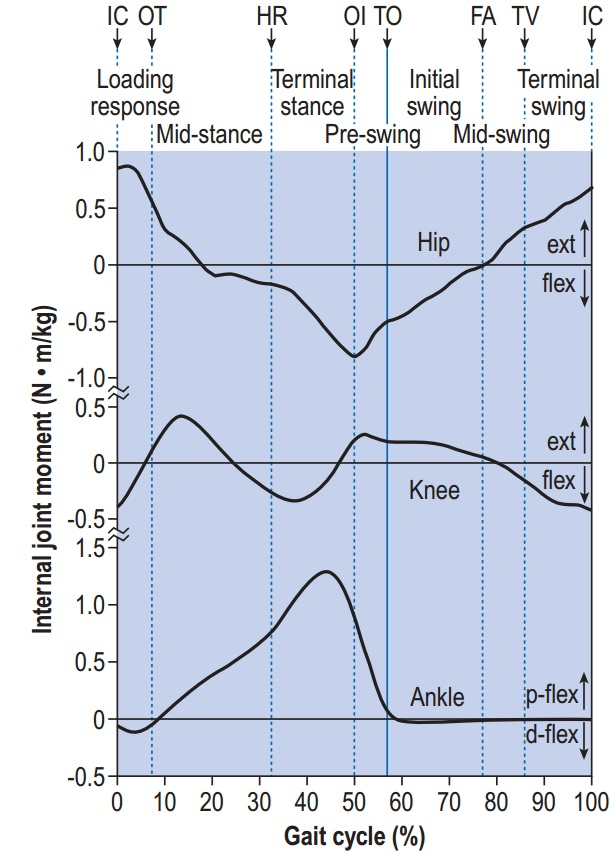
\includegraphics[width=8cm]{fig/f52.jpg}
    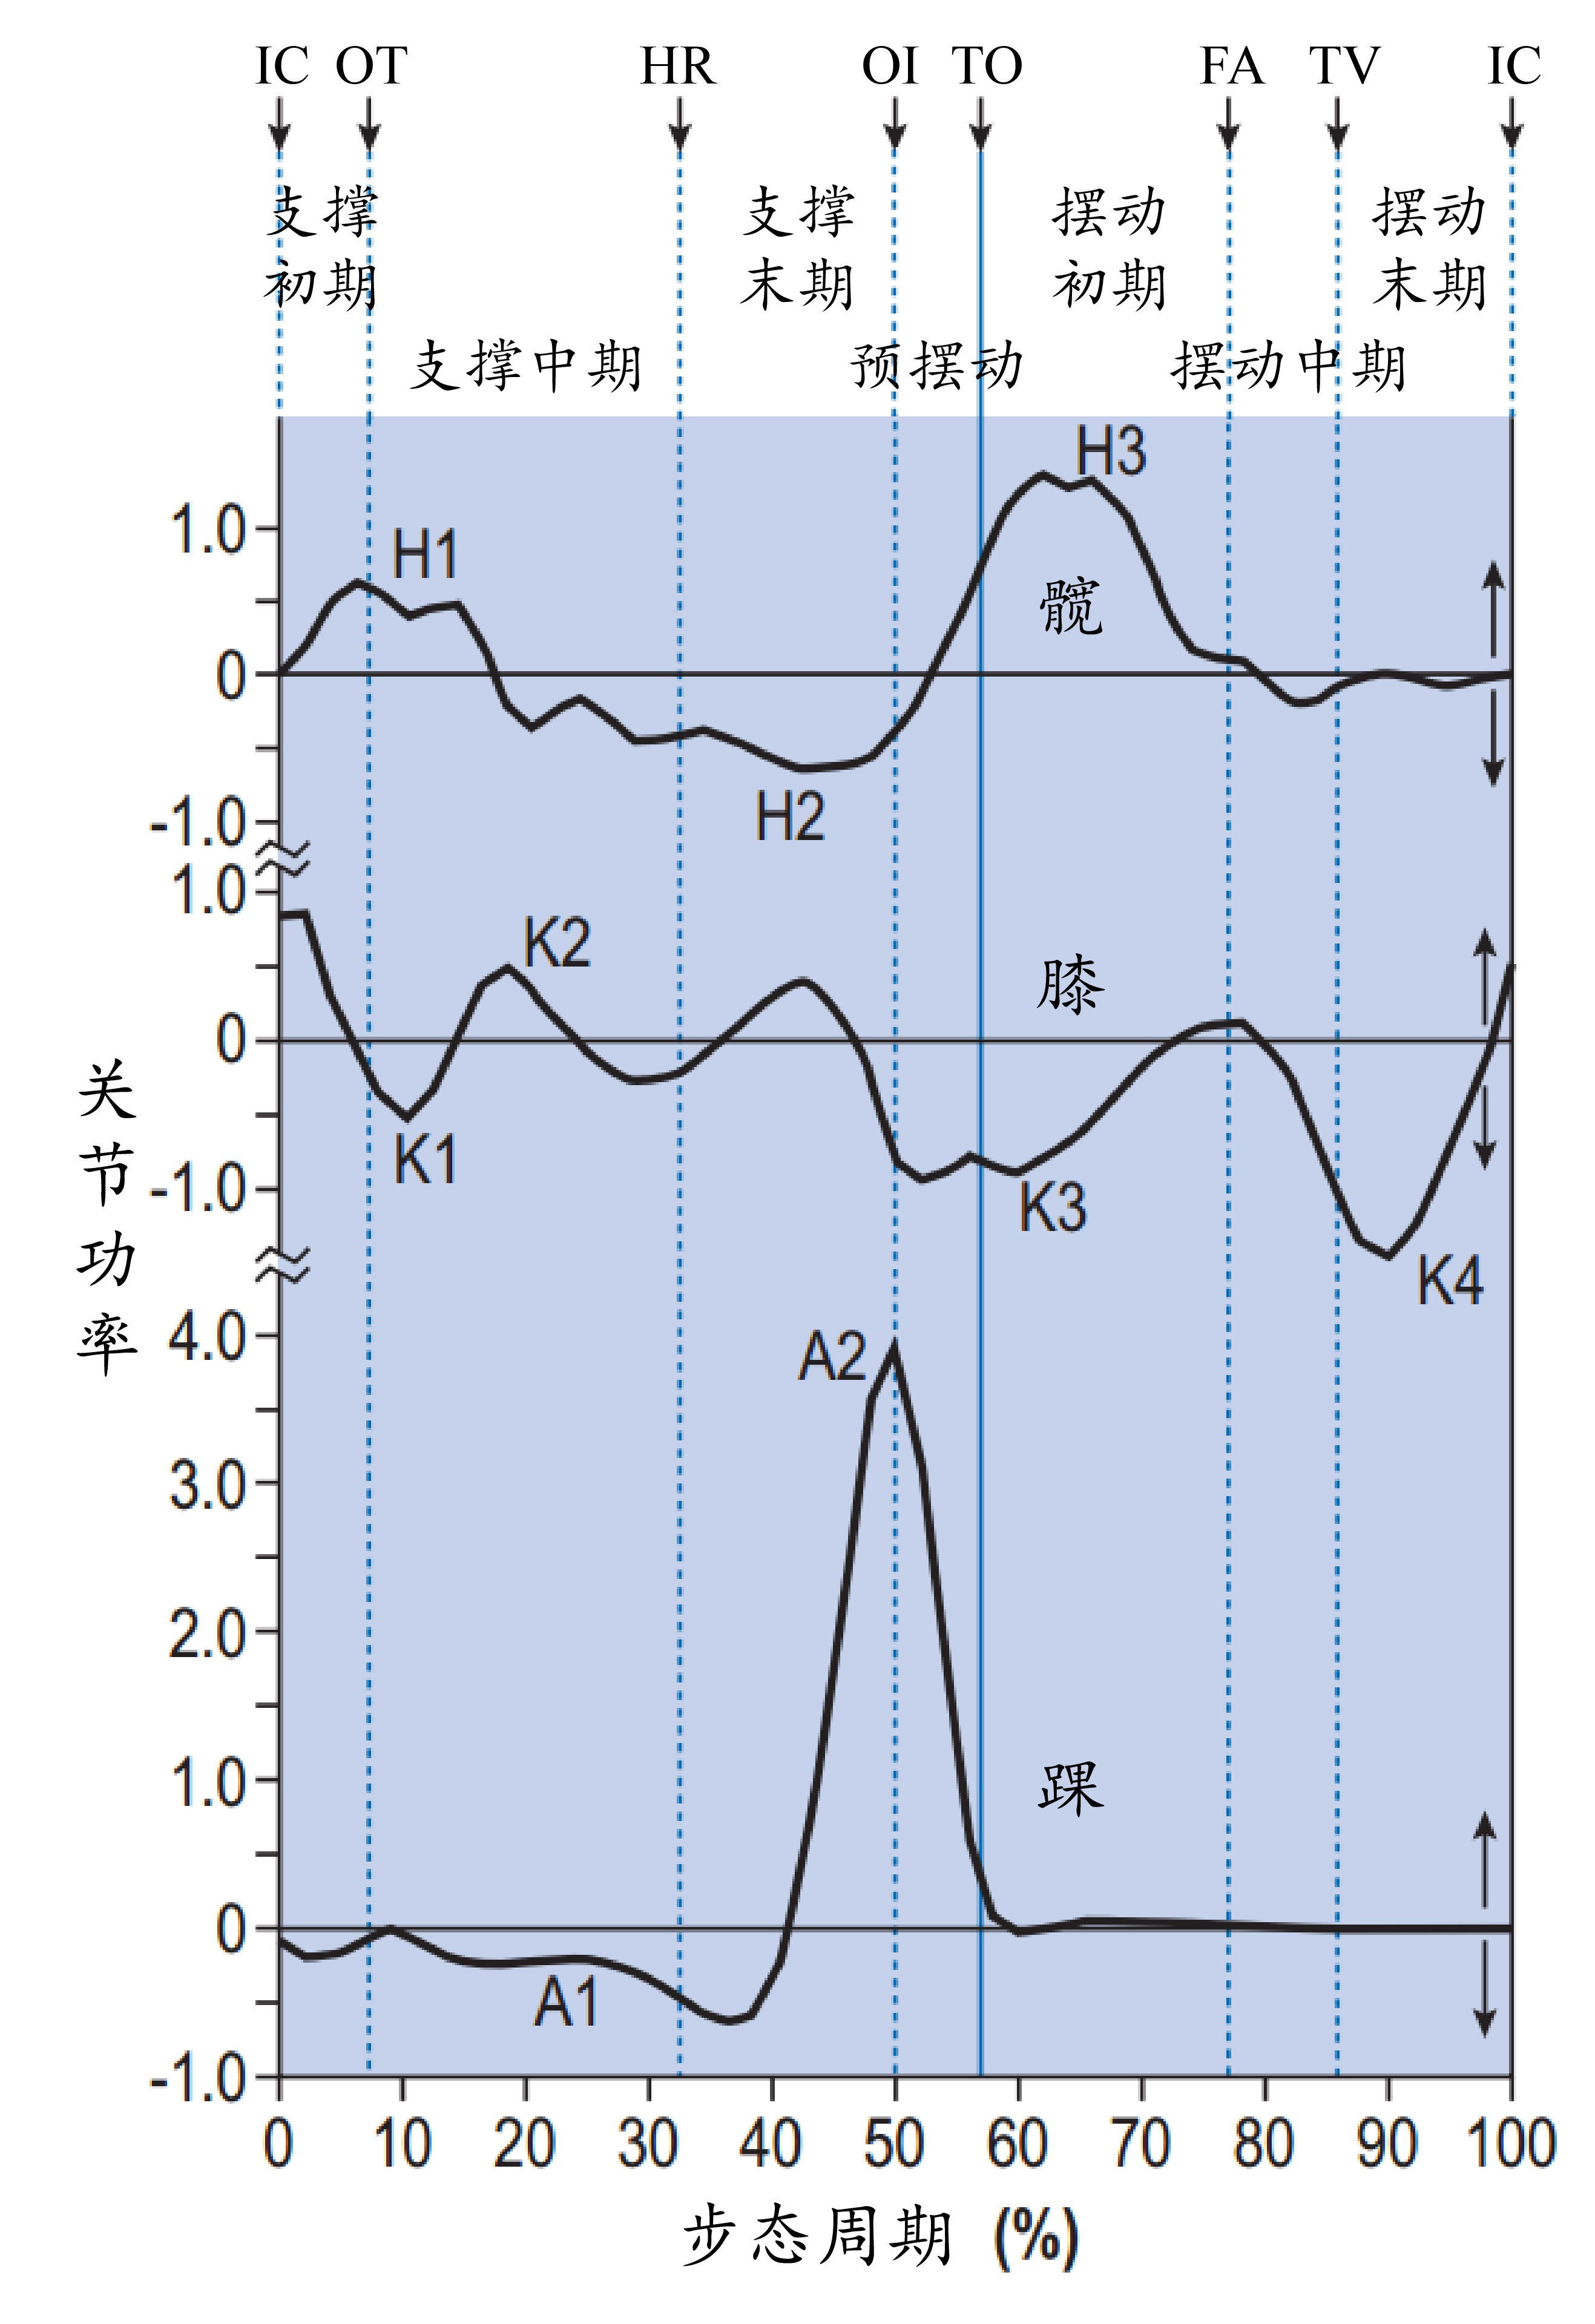
\includegraphics[width=8cm]{fig/f53.jpg}
    \caption{人体行走过程的关节力矩与关节功率\cite{p44}}
    \label{fig:subfigss}
\end{figure}

对于直接力矩控制的理解,可以从人体行走时自身的踝关节力矩出发。如图3.3所示,在步态周期的支撑阶段,踝关节持续施加一个作用力矩,且随着步态周期时间成单调上升和单调下降的过程,并且在即将地面时产生一个较大的关节功率输出。基于时间的直接力矩控制可以看做是一种稳态条件下的助力模式,通过外骨骼的辅助力矩减小人体自身的由肌肉产生的关节力矩,从而提供助力效果。

\begin{figure}[htb]
    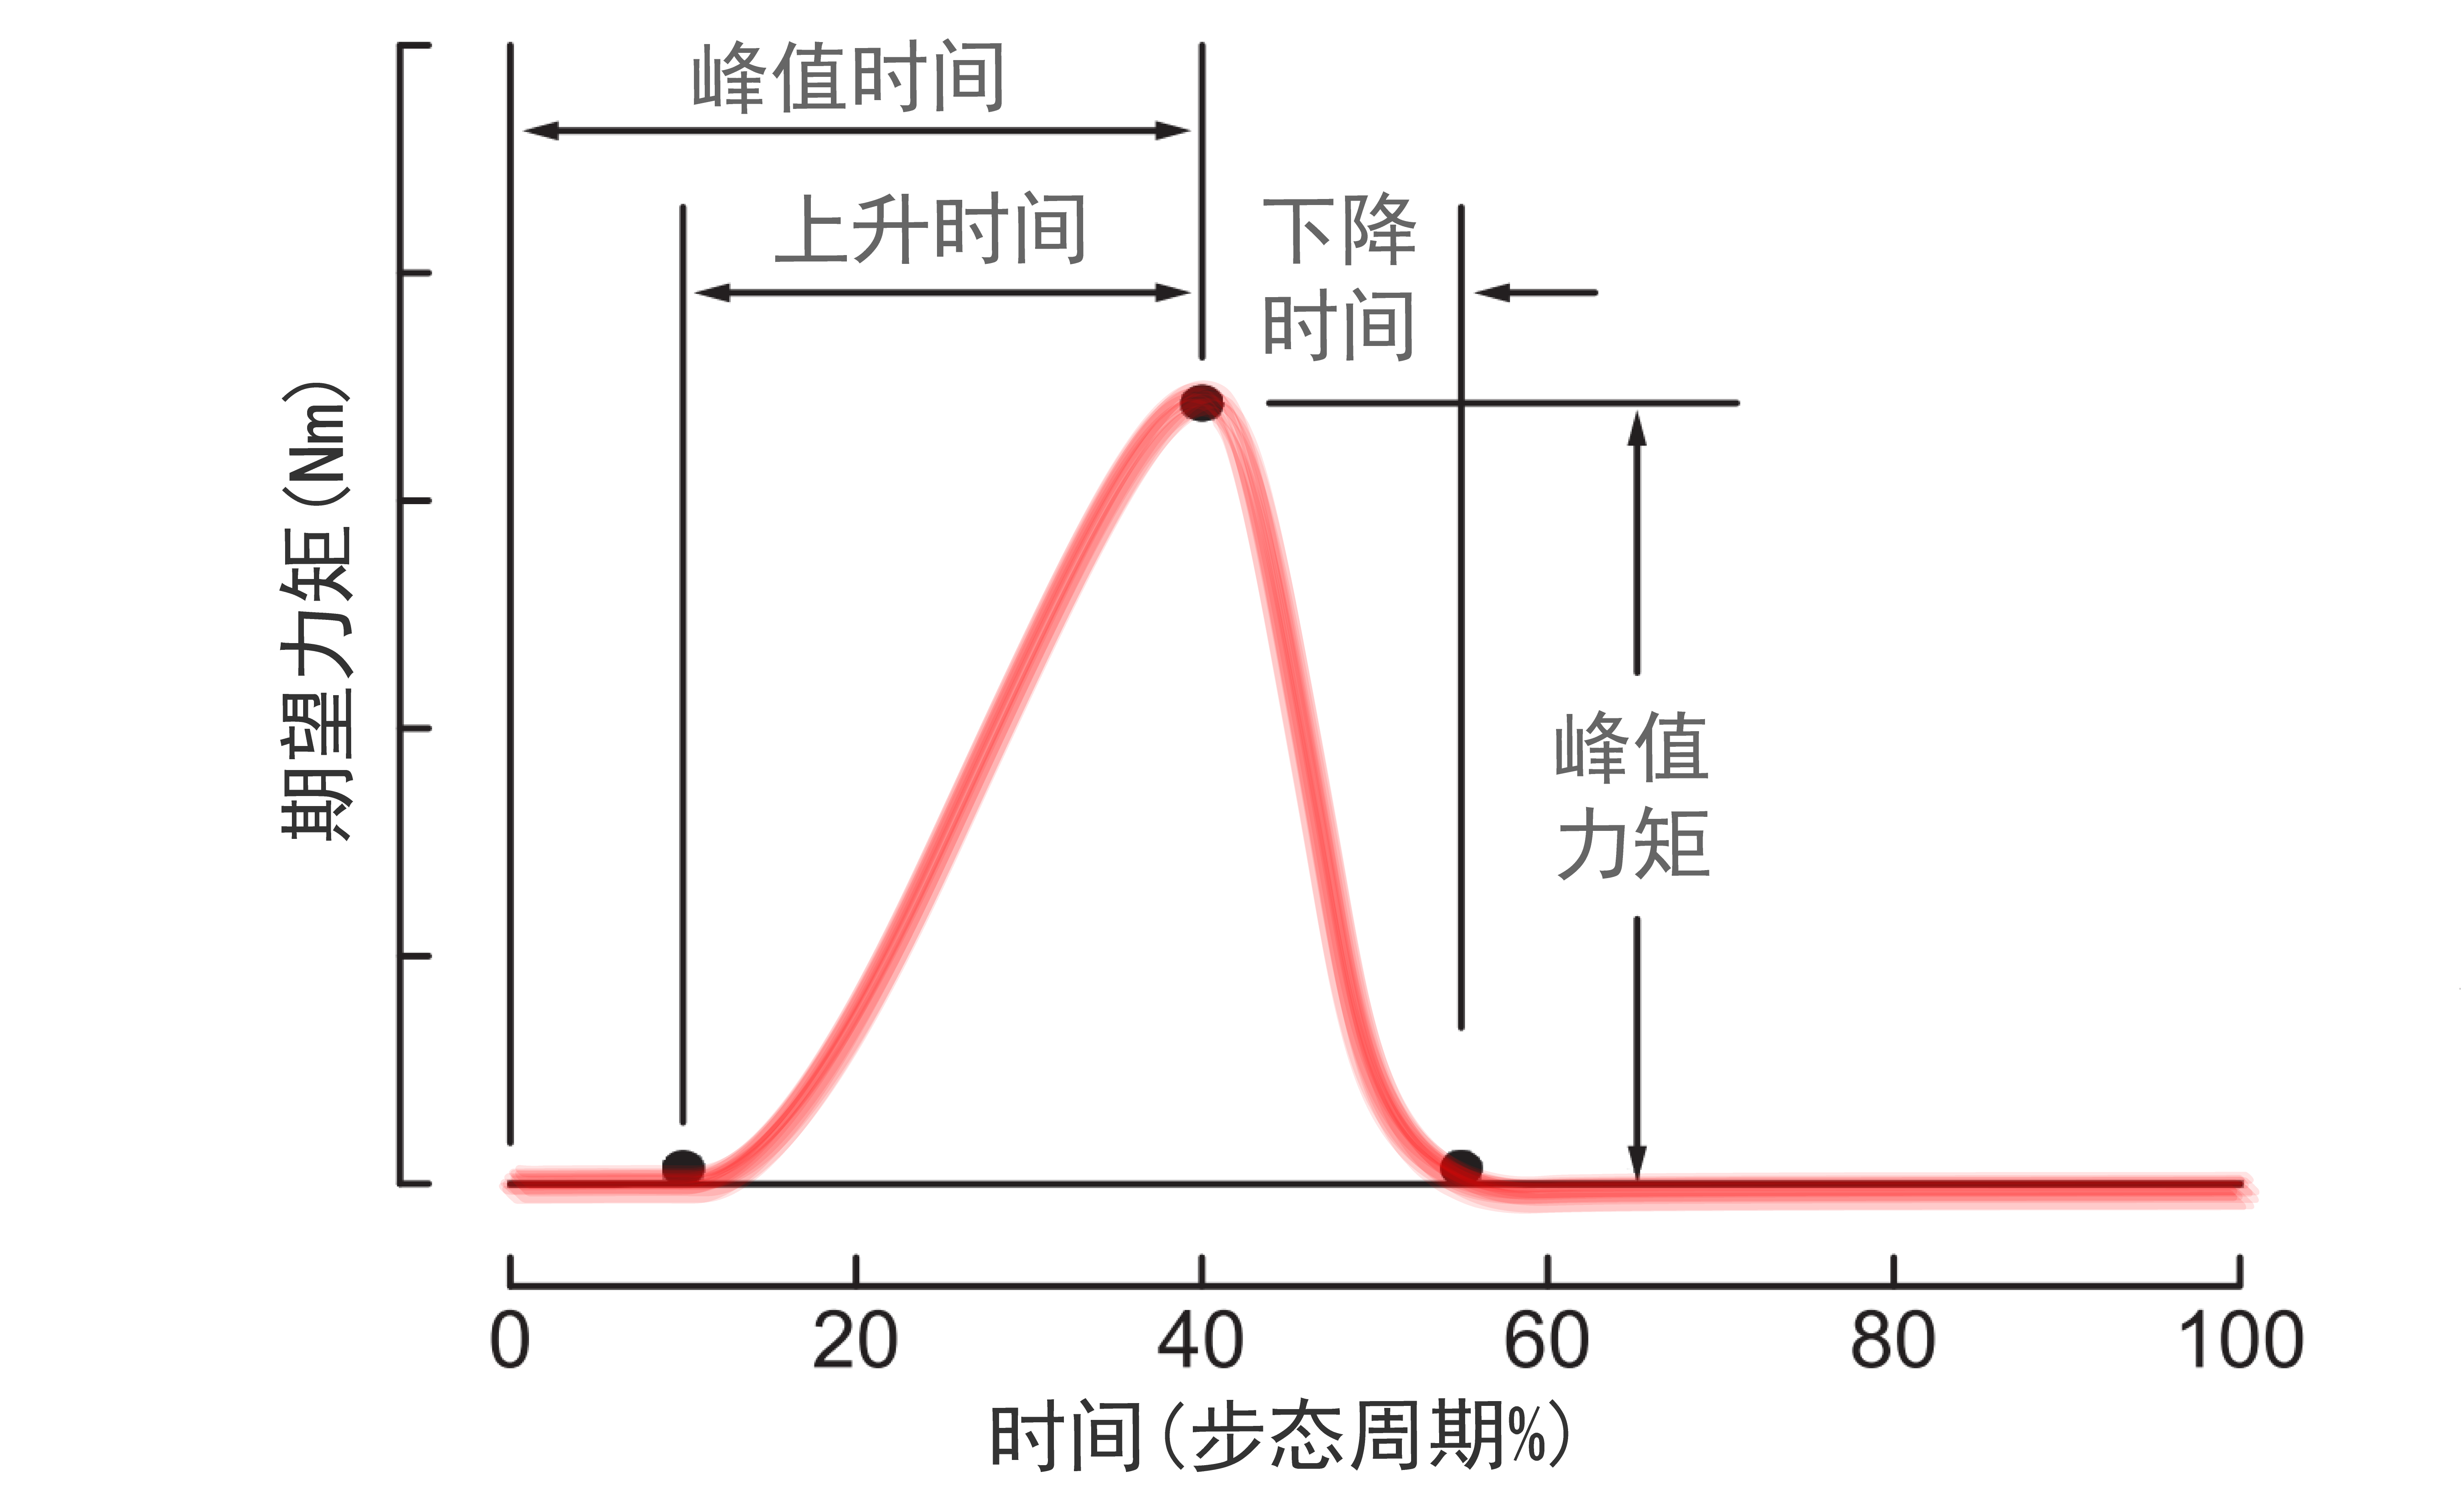
\includegraphics[width=10cm]{fig/f51.png}
    \caption{期望关节力矩曲线}
    \label{fig:mark}
\end{figure}

本文所使用的力矩曲线如图3.4所示。曲线由四个参数确定,分别为:
\begin{enumerate}
    \item 峰值力矩
    \item 峰值时间
    \item 上升时间
    \item 下降时间
\end{enumerate}
其中峰值力矩的单位为N$\cdot$m,三个时间参数的单位均为步态周期的百分比。之后使用三次样条函数对力矩曲线进行插值,从而得到期望力矩的曲线。

由于直接力矩控制反应的是一种稳态条件下的助力模式,一组力矩曲线参数都表示一种独特的助力模式,且适合每个人的助力模式都不尽相同,因此需要针对每个穿戴者配置适合其行走的助力模式。对于本实验的受试者(本文作者),一组适合的助力参数如表3.1所示,后面所有的底层控制实验均在此参数下完成。

\begin{table}[htb]
    \caption[力矩曲线]{力矩曲线参数}
    \begin{tabular}{cccc}
      \toprule
        峰值力矩 & 峰值时间 & 上升时间 & 下降时间 \\
      \midrule
        30 & 45 & 25 & 20 \\
      \bottomrule
    \end{tabular}
\end{table}

\section{底层控制算法设计}
                                                                                        
\subsection{PD反馈控制}

PID控制是控制理论中最常见的控制方法,由于其简单、容易理解、方便调参的特点,广泛的应用在工业系统中。PID控制是反馈控制的一种基本形式,其中P为比例,D为微分,I为微积分。根据实际需求的不同,PID控制器会有多种组合和变形。
\begin{align}
    u(t) = K_p \cdot e(t) + K_d \cdot \dot{e}(t) + K_i\int e(t) dt
\end{align}

PID控制器的三个部分各自具有不同的功能。比例项用来减小误差,代表着反馈控制本质,比例调节的参数$K_p$越大,则误差越小,响应速度越快。但参数过大时控制器会变得不稳定,在阶跃响应时会出现明显的超调现象。微分项的主要作用是减小由比例参数过大导致的超调问题,从二阶模型的角度来看,微分项的加入改变了系统的阻尼,因此微分调节也被称为阻尼调节。在真实的系统中,任何采集的信号都会含有噪声,噪声经微分后会被放大,因此微分项受噪声的干扰较为严重。积分环节主要是来消除稳态误差,在精度要求较高的场合下使用,但会减小系统的稳定性。由于本文所研究的底层控制器的输入信号为时变信号,属于随动跟踪系统,积分环节并不适合,所以最终使用PD控制器进行力矩控制。

\begin{figure}[htb]
    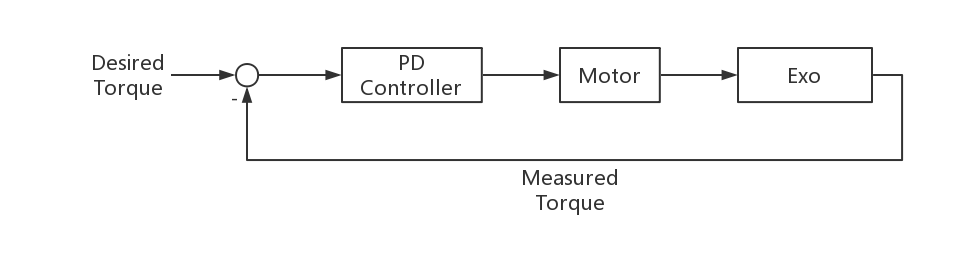
\includegraphics[width=15cm]{fig/f54.jpg}
    \caption{PD反馈控制的系统框图}
    \label{fig:mark}
\end{figure}

控制系统框图如3.5所示,PD控制器根据力矩误差产生电机的控制电压:
\begin{align}
    u(t) = K_p \cdot e(t) + K_d \cdot \dot{e}(t) \\
    e(t) = \tau_{des} - \tau_{real} \\
    \dot e(t) = \dot\tau_{des} - \dot \tau_{real}
\end{align}

\subsection{前馈控制}

将式(3.12)中的$\tau$换为期望力矩$\tau_{des}$可得:
\begin{align}
    \tau_{des} = K_t(\theta_p - \theta_eR)
\end{align}

对上式求导可得:
\begin{align}
    \dot\tau_{des} = K_t(\dot\theta_p - \dot\theta_e R)
\end{align}

整理得:
\begin{align}
    \dot\theta_p = \frac{1}{K_t}\tau_{des} + \dot\theta_e R
\end{align}

进一步忽略$\dot\theta_e R$,并考虑到电机减速比:
\begin{align}
    \dot\theta_m = \frac{N}{K_t}\dot\tau_{des}
\end{align}

带入式(3.5)得:
\begin{align}
    U_a &= \left(\frac{R_{a} f_{e}}{K_{a}}+K_{b}\right) \frac{N}{K_t} \dot\tau_{des} \\
        &= K_o \dot\tau_{des}
\end{align}

因为过程中的许多参数未知,所以参数$K_o$可以通过系统辨识或试错得到。

由于模型的不确定性和建模过程中简化,以单纯的前馈控制无法达到较好的控制效果,一般会与反馈控制相结合构成复合控制。具有前馈控制与PD反馈控制的系统框图如3.6所示。
\begin{figure}[htb]
    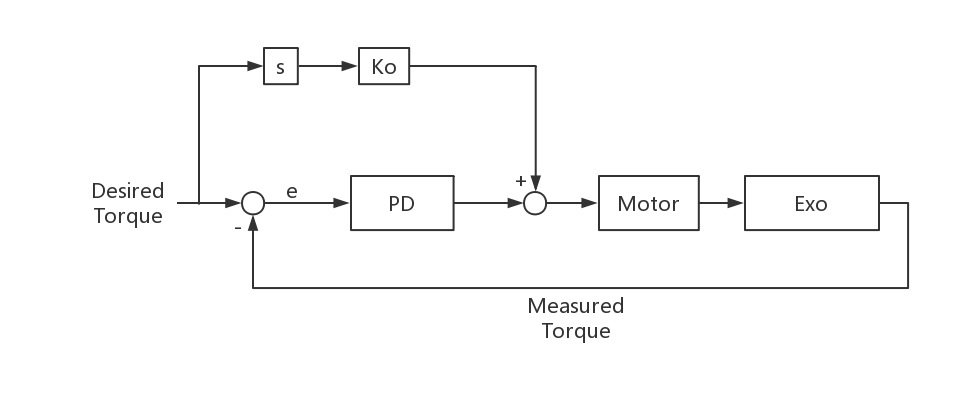
\includegraphics[width=15cm]{fig/f55.jpg}
    \caption{前馈+PD控制的系统框图}
    \label{fig:mark}
\end{figure}

\subsection{迭代学习控制}

迭代学习控制(Iterative Learning Control, ILC)属于智能控制的一种,最早由Uchiyama\cite{p46}于1978年首先提出。该控制方法适合具有重复运动性质的被控对象,它不依赖于系统精确的数据模型,能够以非常简单的方式处理不确定、非线性、强耦合的动态系统,且具有较高的跟踪精度。它通过反复应用先前试验得到的信息,以迭代的形式补偿系统复杂的动力学过程,产生优化输入信号,使系统输出尽可能逼近理想值。虽然步态过程不像工业机器人有固定的循环周期,但在稳定行走时也有着一种周期特性,因此可以使用迭代学习进行力矩控制。

本文采用Arimoto\cite{p47}提出的$D$型迭代学习控制律,假设外骨骼系统在第$n$个步态循环的第$i$个时刻力矩跟踪的误差为$e(i,n)$:
\begin{align}
    e(i,n) = \tau_{res} - \tau_{real}
\end{align}

迭代学习控制器根据$e(i,n)$通过周期迭代的方式学习一个输出序列$u(i,n)$,每个运动周期结束时更新一次迭代:
\begin{align}
    u(i,n+1) = u(i,n) + K_l\dot{e}(i+D,n)
\end{align}

其中参数$D$考虑了延时问题,$K_l$为迭代学习的误差学习参数。

迭代学习控制可以作为一个独立的控制器,也可以与其他控制器组合使用。单纯的ILC无法对抗扰动甚至胡不稳定,因此较多的将ILC与PD控制相结合,PD控制进行扰动抑制,ILC用于消除反馈控制所残留的轨迹跟踪误差,从而使跟踪达到更高的精度。

\section{踝关节外骨骼力矩控制实验}

本文对上一小节所提出的三种控制算法,设计了如下四种控制器形式,并进行了实验和对比:
\begin{enumerate}
    \item PD控制
    \item PD控制+前馈控制
    \item ILC
    \item PD控制+前馈控制+ ILC
\end{enumerate}

\begin{table}[htb]
    \caption[控制参数]{三种控制算法的参数值}
    \begin{tabular}{ccccc}
      \toprule
        $K_p$ & $K_d$ & $K_o$ & $K_l$ & $D$ \\
      \midrule
        5 & 0.4 & 1 & 2 & 9 \\
      \bottomrule
    \end{tabular}
\end{table}


三种控制算法都需要进行参数整定以达到较好的控制效果。对PD控制器的参数本文使用曲线响应法进行整定,对于前馈控制和ILC的参数使用试错法。三种控制算法的最终参数如表3.2所示。

力矩控制实验时,受试者穿戴外骨骼以1.25m/s的速度在跑步机上稳定的行走。其中无ILC的控制器在参数调整一分钟后开始记录数据,含有ILC的控制器在学习稳定后开始记录。每个控制器记录两分钟,约120步的数据。

\begin{figure}[htb]
    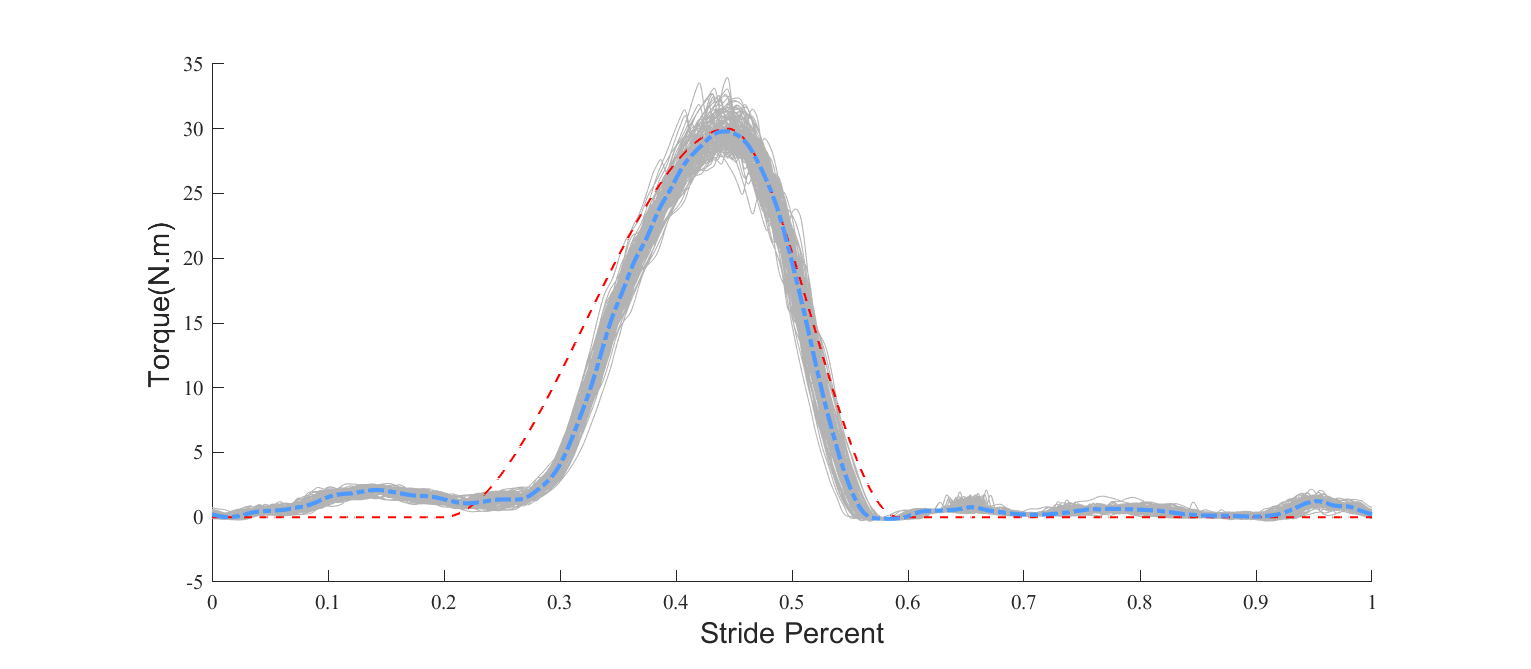
\includegraphics[width=17cm]{fig/f56.eps}
    \caption{PD控制的力矩跟踪效果}
    \label{fig:mark}
\end{figure}
\begin{figure}[!htb]
    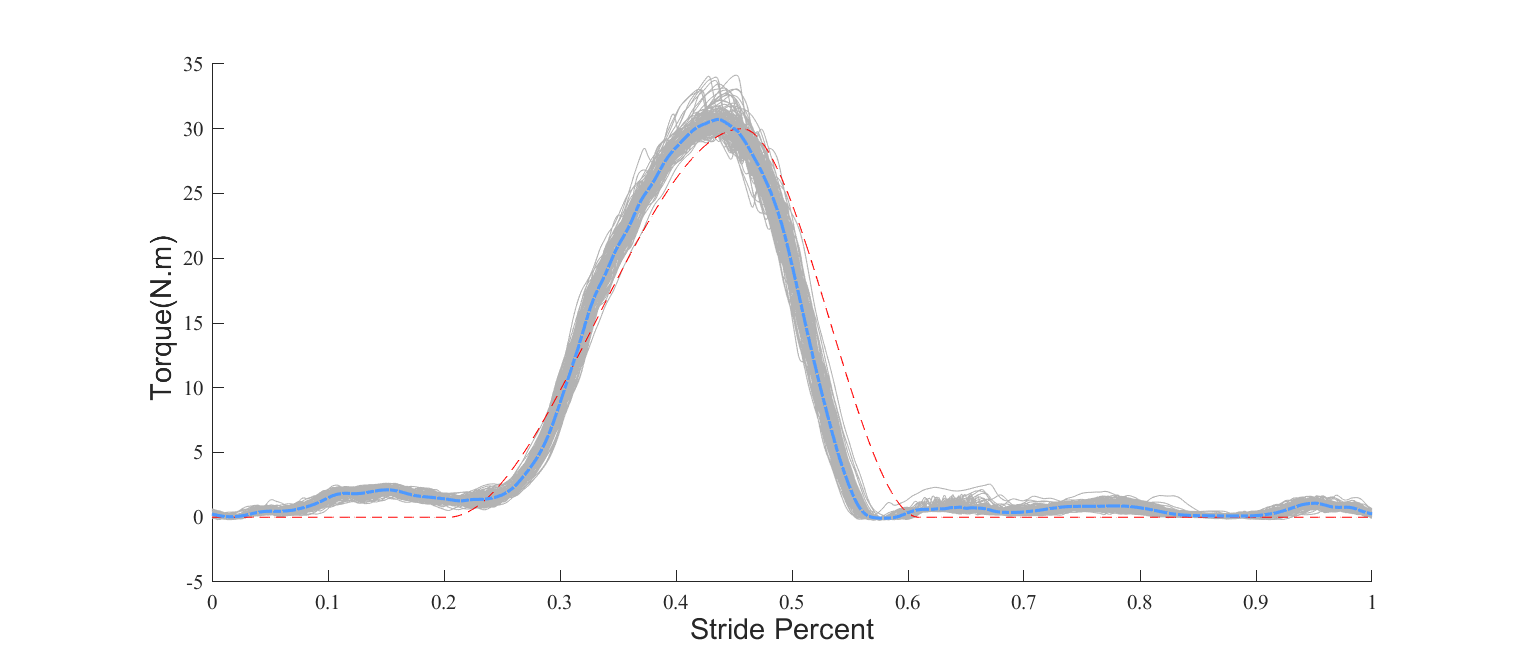
\includegraphics[width=17cm]{fig/f57.eps}
    \caption{PD +前馈控制的力矩跟踪效果}
    \label{fig:mark}
\end{figure}

\begin{figure}[!htb]
    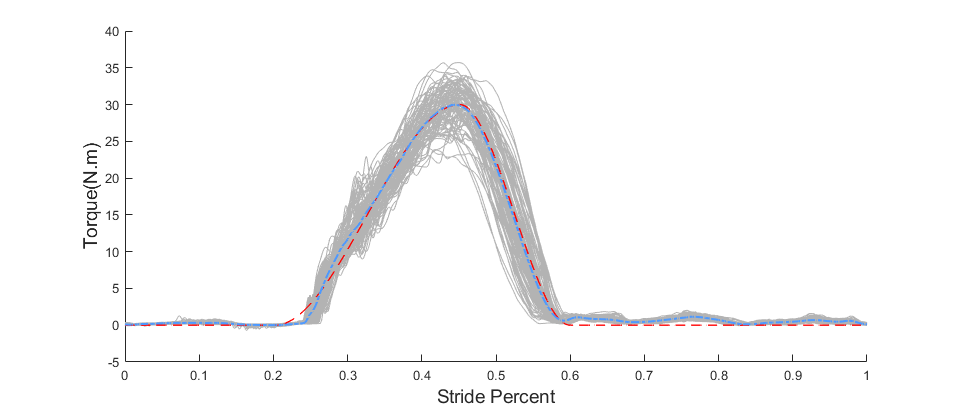
\includegraphics[width=17cm]{fig/f58.png}
    \caption{ILC的力矩跟踪效果}
    \label{fig:mark}
\end{figure}
\begin{figure}[!htb]
    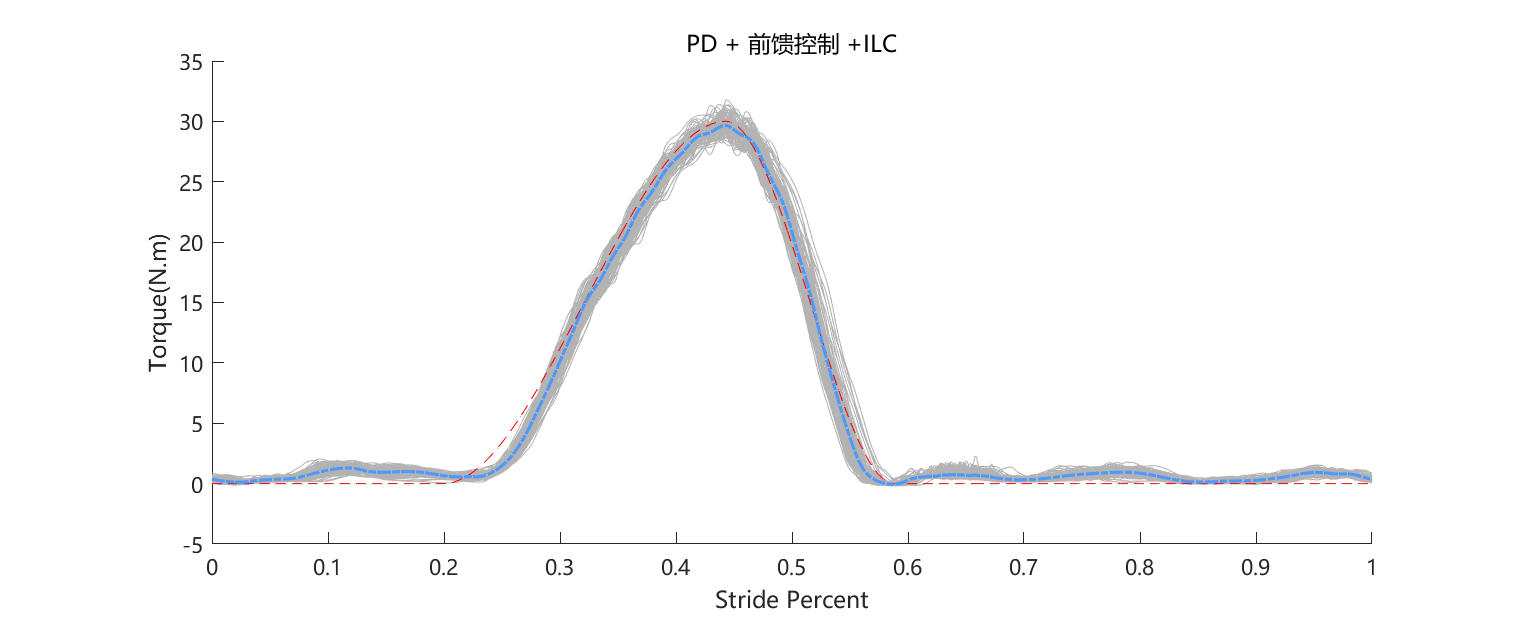
\includegraphics[width=17cm]{fig/f59.eps}
    \caption{PD +前馈+ ILC的力矩跟踪效果}
    \label{fig:mark}
\end{figure}

\begin{table}[!htb]
    \caption[控制参数]{四种种控制器力矩追踪的均方根误差}
    \begin{tabular}{cccc}
      \toprule
        PD & PD +前馈 & ILC控制 & PD +前馈+ ILC \\
      \midrule
        2.226 & 1.729 & 1.605 & 0.968 \\
      \bottomrule
    \end{tabular}
\end{table}

实验结果如图3.7-3.10所示,图中红色虚线为期望力矩曲线,灰色实线为每一步实际的跟踪结果,蓝色实线为平均力矩跟踪结果,表3.3为四种控制器力矩跟踪的均方根误差。

由图3.8可以看出,加入前馈控制后力矩曲线上升阶段追踪效果较PD控制好,但在下阶段有较大误差,这可能是源于鲍登线拉和松两种状态的非线性。迭代学习控制平均的追踪效果较好,但对于扰动的抑制能力较差,因此每一步的力矩跟踪波动较大。PD、前馈、ILC组合在一起时有相对较好的控制效果,追踪精度较高且波动范围较小。

\section{本章小结}

本章研究了外骨骼力矩控制方法。力矩控制由上层控制器与底层控制器组成,上层控制器用来产生期望力矩曲线,底层控制器实现对期望力矩曲线的跟踪。针对上层控制器,本文采用基于时间的直接力矩控制器,通过三次函数插值得到期望力矩曲线。针对底层控制器,本文提出了三种控制算法,设计了四种不同组合形式的控制器,并对其进行了验证与对比。实验结果表明,综合三种算法的控制器具有较好的力矩追踪效果。